\section{Cross-Validation (CV)}
a technique to compare (and select from) different models (=different parameter values) \\

\textbf{Use Cases}

\begin{itemize}
    \item Obtain a \textcolor{blue}{better estimate of the generalization error}
    \item Selection of hyper parameters, split/train pattern of cross validation can be used to \textcolor{blue}{find optimal hyper parameters} (Parameter der Training Prozedur, e.g. $\lambda$)
\end{itemize}
\vspace{10pt}
\textbf{Problem with (80/20) Data Separation}
\begin{itemize}
    \item Test Error depends on random set
    \item For different sets, the test error would be different
\end{itemize}
\vspace{10pt}
Without cross-validation

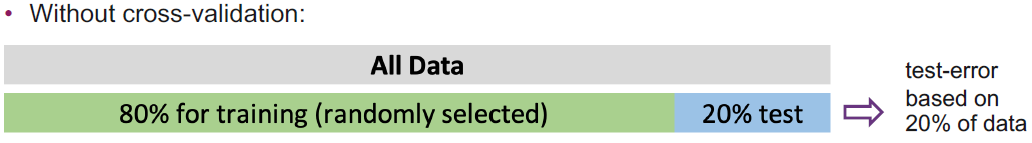
\includegraphics[width=\linewidth]{k_fold.png}

\subsection{k-fold Cross-Validation}

With k-Fold Cross-Validation\\

\begin{itemize}
    \item The data is split once into k folds
    \item Repeats the split-train-test procedure k times, using a systematic resampling procedure
    \item Then train/test is repeated k-times.
    \item Each fold participates in \textcolor{blue}{k-1 training phases} and is used \textcolor{blue}{once for testing}
\end{itemize}

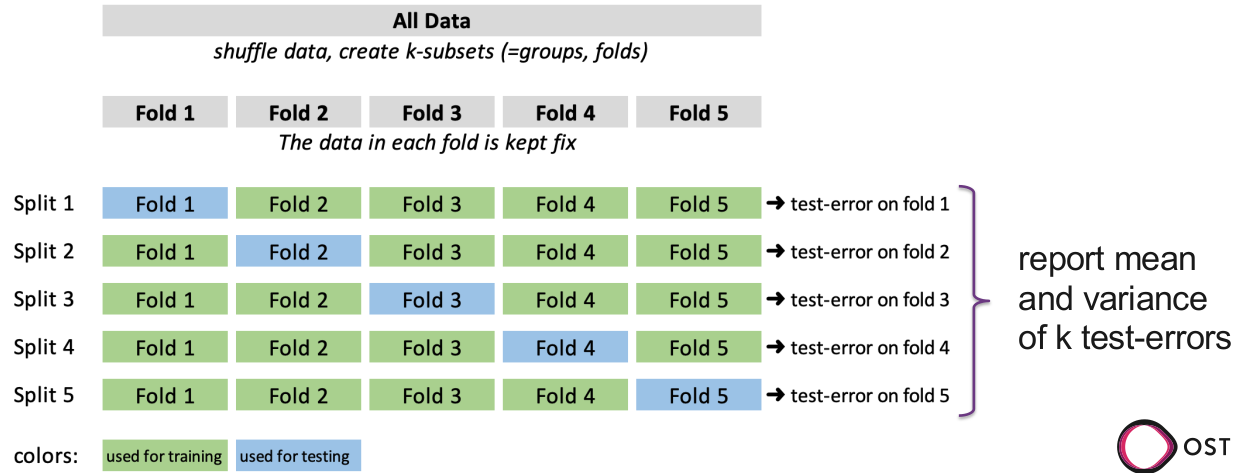
\includegraphics[width=\linewidth]{k_fold2.png}

\begin{itemize}
    \item Typical Values for k are 5, 10 or N
    \item The data of a fold does not change during procedure
    \item Do not preprocess the whole dataset, but apply the preprocessing pipeline (standardization) to each split
    \item Each split generates a different model
    \item With regularization, each split may yield a different  model and a different optimal $\lambda$
\end{itemize}

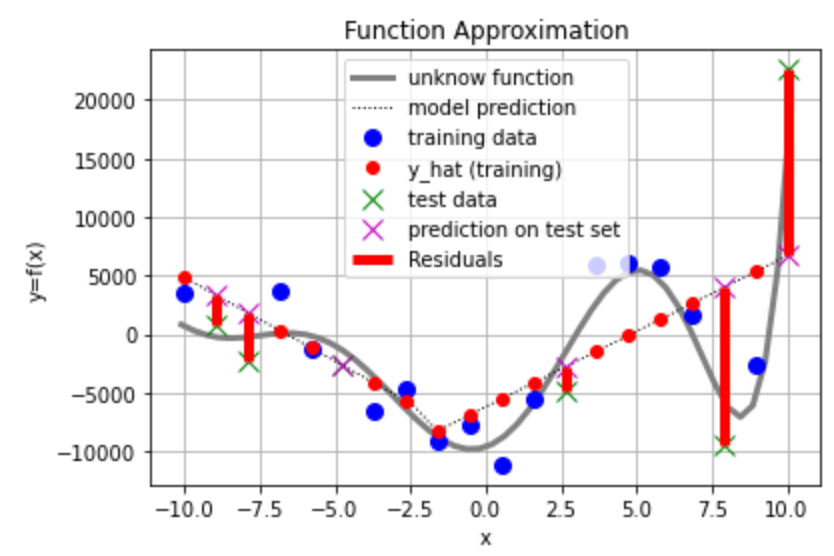
\includegraphics[width=\linewidth]{learning-model.png} \\
\columnbreak

\textbf{Compare results}

Anwendung des zweiten Use Cases (Use Case 1 mit unterschiedlichen $\lambda$ berechnet und \textcolor{blue}{MSE} vergleichen)

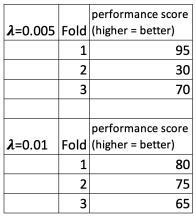
\includegraphics[width=0.5\linewidth]{compare-folds.png}

$220/3 > 195/3$ results in better regularization of $\lambda_{opt} = 0.01$

Anschliessend $\lambda_{opt}$ in allen Modell für \textcolor{blue}{alle Trainingsdaten verwenden}

\subsection{Scikit-learn}

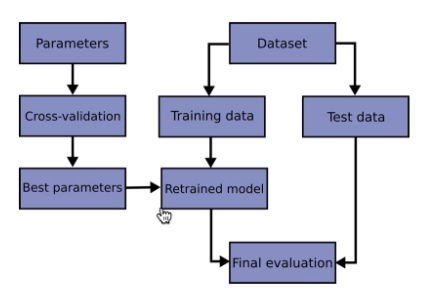
\includegraphics[width=\linewidth]{scikit.png}
